\documentclass{article}
\usepackage{ifxetex}
\usepackage{ifxetex}
\ifxetex
  \usepackage{fontspec}
\else
  \usepackage[T1]{fontenc}
  \usepackage[utf8]{inputenc}
  \usepackage{lmodern}
  \usepackage{float}
  \usepackage{amssymb}
  \usepackage{amsmath}
  \usepackage{amsmath}
  \usepackage{graphicx}
  \usepackage{morefloats}
  \usepackage{wrapfig}
  \usepackage[top=1in, bottom=1.25in, left=1.1in, right=1.1in]{geometry}
  \usepackage[dvipsnames]{xcolor}
  \usepackage{enumerate}
\fi

\begin{document}
\begin{titlepage}
\begin{center}
    \vspace*{-1in}
    \begin{figure}[htb]
    \begin{center}
    
\includegraphics[width=8cm]{escudo-gde-trans.png}
    \end{center}
\end{figure}
\begin{center}
LICENCIATURA EN FÍSICA \\
\vspace*{0.15in}
DEPARTAMENTO DE FÍSICA \\
\vspace*{0.6in}
\begin{large}
FÍSICA COMPUTACIONAL 1 \\
\end{large}
\vspace*{0.2in}
\rule{80mm}{0.1mm}\\
\vspace*{0.1in}
\begin{large}
\textbf{Evaluacion 2\\ }
\end{large}
\vspace*{0.3in}
\begin{large}
Alumna: \\
\vspace*{0.1in}
Brambilla Zamorano Fátima Fernanda\\
\end{large}
\vspace*{0.3in}
\rule{80mm}{0.1mm}\\
\vspace*{0.1in}
\begin{large}
Fecha: \\ 26/04/18\\
\end{large}
\end{center}
\end{center}
\end{titlepage}

\section {Reporte de Actividad}

\subsection {Objetivo 1}
Esta evaluación trato de recrear el \textit{Atráctor de Lorenz}, el cual es un ejemplo de \textit{caos dinámico}. Para esto, se nos proporciono un código para Python, el cual tomaríamos para recrearlo en nuestro notebook en Jupyter Lab, al tiempo que sería analizado para ver como funcionaba.
Una vez hecho esto, debíamos cambiarle los parámetros \textit{sigma, rho y beta}, para ver cual era el comportamiento esperado del atráctor con diferentes parámetros dentro de sus condiciones iniciales.
A continuación se mostraran algunas partes del código original, y las gráficas que este mostraba una vez que era copilado.
\begin{figure}[H]
    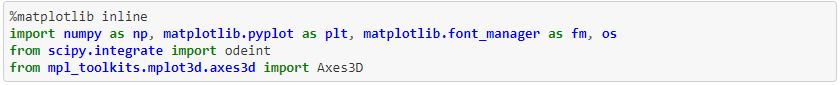
\includegraphics[width=1\textwidth]{Celda1.PNG}
    \centering
    \label{Cod}
\end{figure}
En está primera celda que se muestra arriba, simplemente se han importado diferentes bibliotecas al programa, las cuales serán necesarias para resolver el sistema de Lorenz.
En la siguiente celda que se muestra, se han definido parámetros con los que el sistema trabajara, siendo estos los mencionados al principio del documento. Además, se define un tiempo de inicio y final, así como un número de puntos en el lapso de tiempo definido, que son donde se resolverá el sistema.
\begin{figure}[H]
    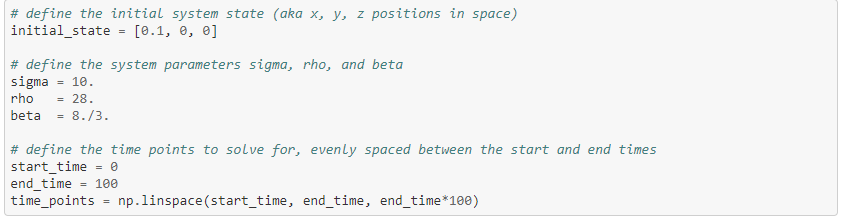
\includegraphics[width=1\textwidth]{Celda2.PNG}
    \centering
    \label{Cod}
\end{figure}
En las siguientes fracciones de código, se muestra como se definió el sistema de ecuaciones ordinarias que modelan el atráctor de Lorenz, también se muestra en la segunda parte, la función odeint(), la cual se usa para resolver sistemas de ecuaciones diferenciales ordinarias.
En la segunda imagen se puede ver la manera en que se procedió para "armar" la gráfica que muestra el comportamiento del atráctor.
Lo que se puede mencionar de estas dos partes del código, es que en el caso de la celda que se muestra en primer lugar, en ella se utilizan elementos que ya habíamos prácticado antes en el curso, mientras que en la celda que se muestra en la segunda imagen, es que se gráfica en tres dimensiones, algo que no habíamos hecho hasta el momento.
Por ello es importante que analicemos bien la manera en que se gráfico este comportamiento, pues es posible que más adelante en nuestro paso por la carrera, necesitemos hacer gráficasd e ese mismo estilo.
\begin{figure}[H]
    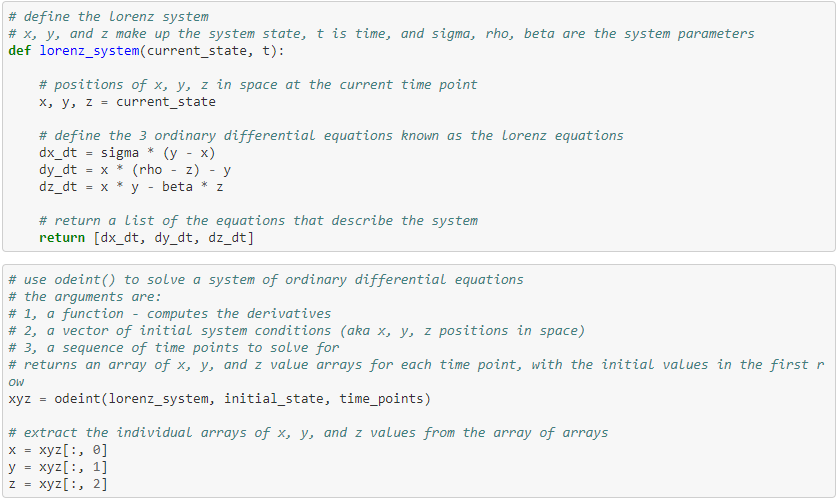
\includegraphics[width=1\textwidth]{Celda3.PNG}
    \centering
    \label{Cod}
\end{figure}
\begin{figure}[H]
    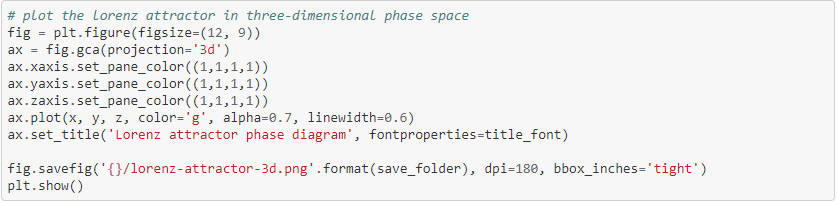
\includegraphics[width=1\textwidth]{Celda4.PNG}
    \centering
    \label{Cod}
\end{figure}
Y la imagen que nos gráfica el código en la última celda mostrada, es la siguiente:
\begin{figure}[H]
    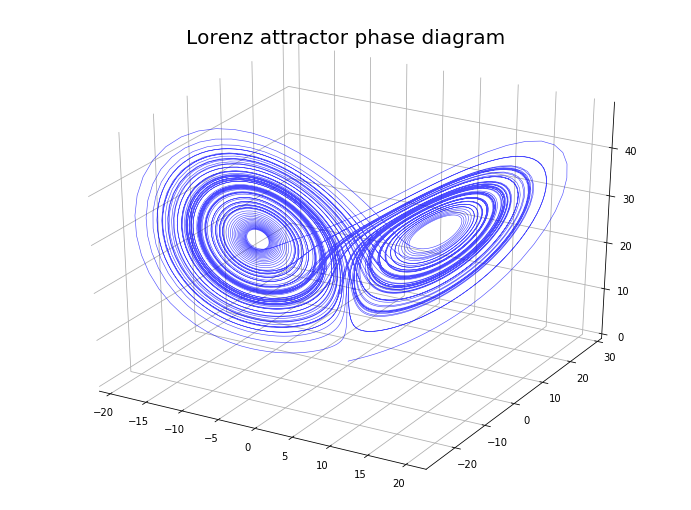
\includegraphics[width=0.5\textwidth]{Visualizacion1.png}
    \centering
    \label{Graf}
\end{figure}
Pero, ver su comportamiento en tres dimensiones no siempre nos deja en claro como es que se mueve, por ello es que a continuación se muestra como se gráficaron los comportamientos para los distintos planos del espacio
\begin{figure}[H]
    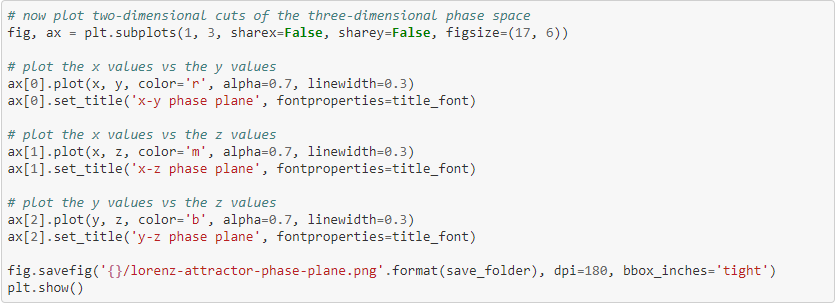
\includegraphics[width=1\textwidth]{Celda5.PNG}
    \centering
    \label{Cod}
\end{figure}
Y las gráficas arrojadas por este código son la siguientes:
\begin{figure}[H]
    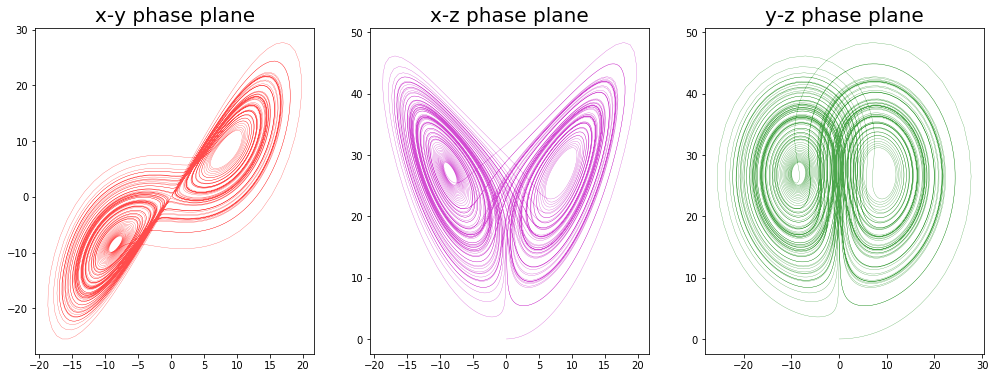
\includegraphics[width=0.8\textwidth]{GraficaTriples1.png}
    \centering
    \label{Grad}
\end{figure}

Hacer estas gráficas fue la primera parte de la actividad, y de manera adicional, se nos pedía que se hiciera un gráfico que mostrara el comportamiento de las distintas variables involucradas (x, y, y z) en función del tiempo. Para esto, se uso el siguiente código:
\begin{figure}[H]
    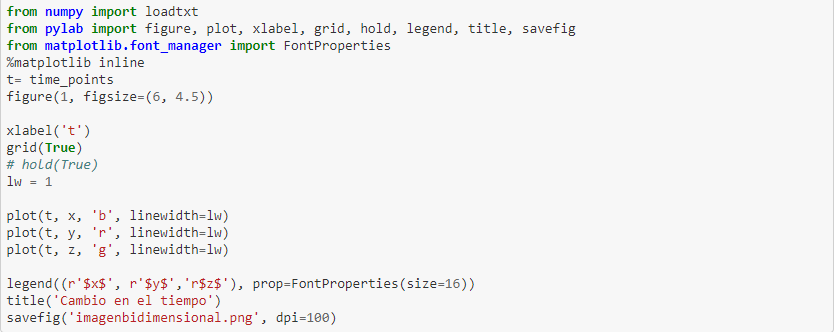
\includegraphics[width=1\textwidth]{Celda6.PNG}
    \centering
    \label{Cod}
\end{figure}
Las imagen creada es esta:
\begin{figure}[H]
    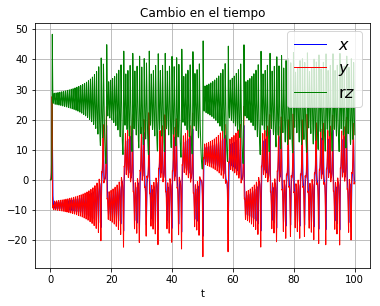
\includegraphics[width=0.5\textwidth]{Grafica1.png}
    \centering
    \label{Grad}
\end{figure}
Sin embargo, en esta no es posible ver del todo bien el comportamiento de la variable x, el cual esta marcado por la linea azul, por ello es que se usaron limites en para poder ver mejor el comportamiento de esta. Mediante el siguiente fragmento:
\begin{figure}[H]
    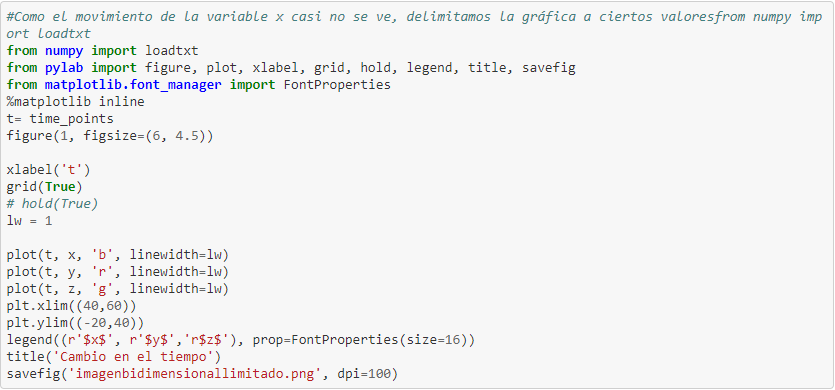
\includegraphics[width=1\textwidth]{Celda7.PNG}
    \centering
    \label{Cod}
\end{figure}
Obteniendo la siguiente imagen:
\begin{figure}[H]
    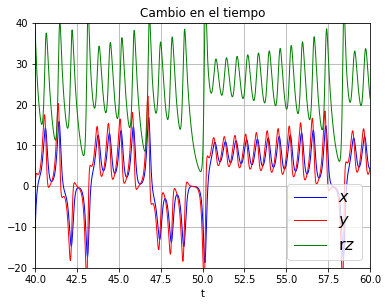
\includegraphics[width=0.5\textwidth]{Grafica2.png}
    \centering
    \label{Grad}
\end{figure}
En esta imagen es fácil ver que el comportamiento de x y y es casi el mismo, de modo que sus lineas de movimientos están una sobre la otra.

En segundo lugar, para la primera parte del examen, que consitía en repetir el código de Geoff Beoing, teníamos que hacer una animación del atráctor de Lorenz, la cual también fue proporcionada, y se verá a continuación el código que crea dicha animación.
\begin{figure}[H]
    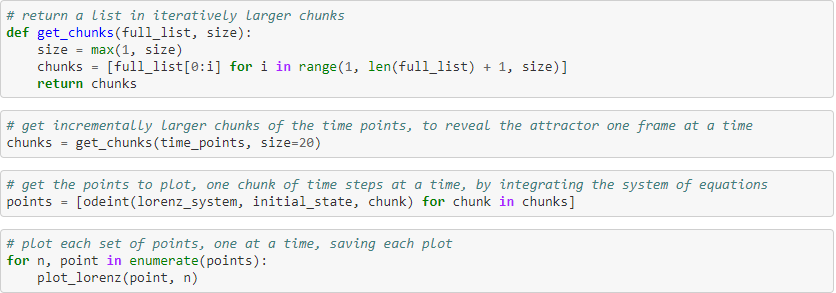
\includegraphics[width=1\textwidth]{Celda8.PNG}
    \centering
    \label{Cod}
\end{figure}
\begin{figure}[H]
    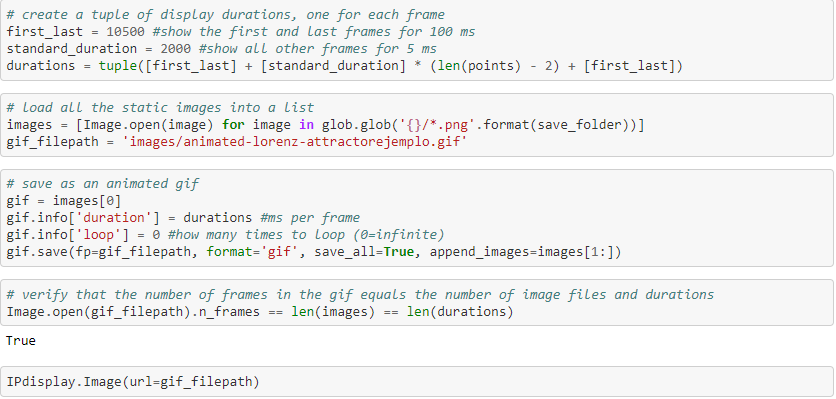
\includegraphics[width=1\textwidth]{Celda9.PNG}
    \centering
    \label{Cod}
\end{figure}
Sin embargo, la animación no puede ser mostrada ni en github ni aquí, sin embargo, al momento de correr el código en Python, se puede perfectamente.

\subsection {Objetivo 2}
En segundo lugar, se nos pidió que observáramos el comportamiento del atráctor de Lorenz con distintos valores para los parámetros sigma, rho y beta.
Los cuales se muestran a continuación en el primer caso, seguidos de sus gráficas en tres dimensiones, y las gráficas para los planos.
\begin{figure}[H]
    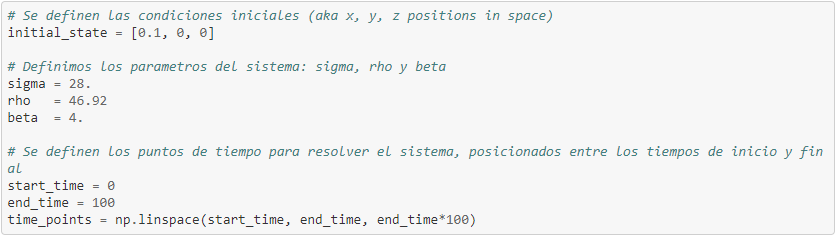
\includegraphics[width=1\textwidth]{Celda10.PNG}
    \centering
    \label{Cod}
\end{figure}
\begin{figure}[H]
    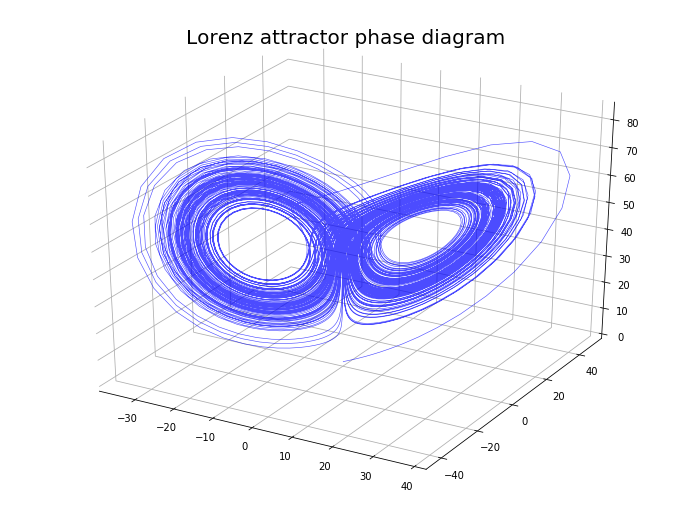
\includegraphics[width=0.5\textwidth]{Visualizacion2.png}
    \centering
    \label{Grad}
\end{figure}
\begin{figure}[H]
    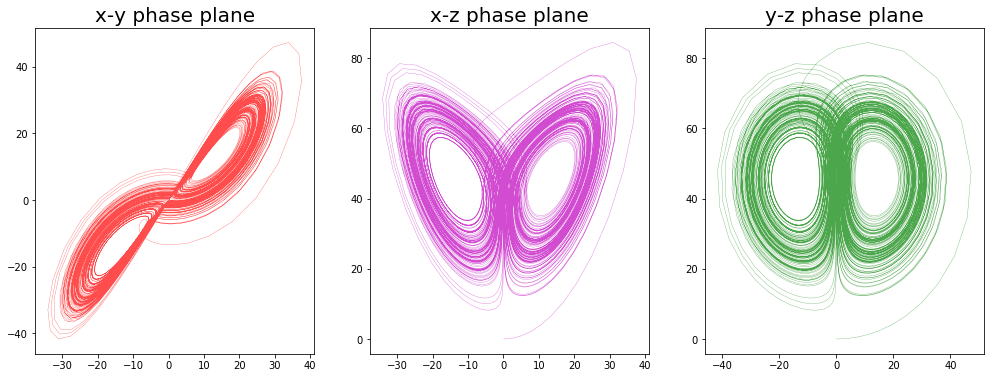
\includegraphics[width=0.8\textwidth]{GraficasTriples2.png}
    \centering
    \label{Grad}
\end{figure}
Como en el objetivo uno, también debíamos crear una animación de este comportamiento, sin embargo, el código es exactamente el mismo, de modo que no se mostrará de nuevo en el documento.
Por último, había que analizar el comportamiento del sistema en con otros parámetros, los cuales se muestran a continuación, seguido de las gráficas proporcionadas:
\begin{figure}[H]
    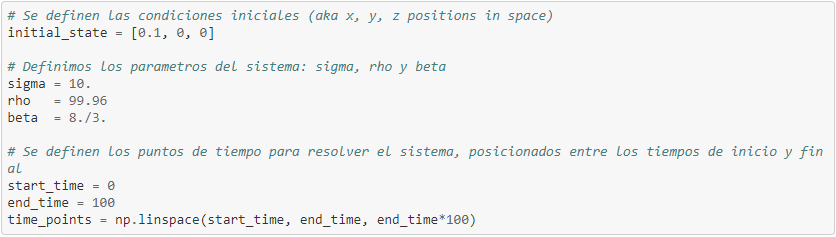
\includegraphics[width=1\textwidth]{Celda11.PNG}
    \centering
    \label{Cod}
\end{figure}

\begin{figure}[H]
    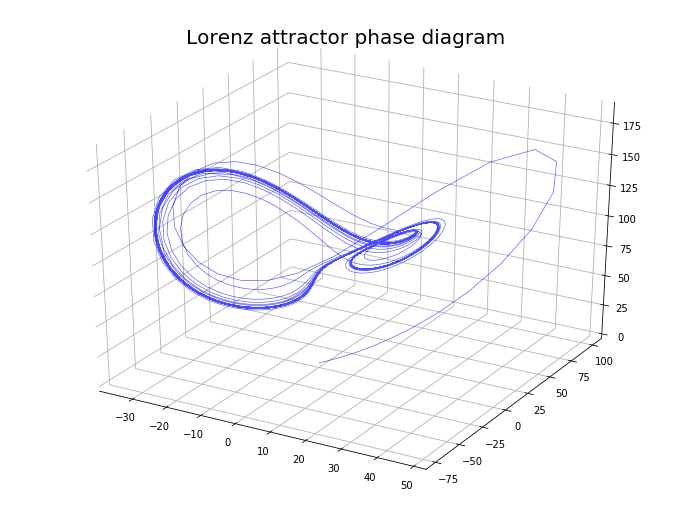
\includegraphics[width=0.5\textwidth]{Visualizacion3.png}
    \centering
    \label{Grad}
\end{figure}

\begin{figure}[H]
    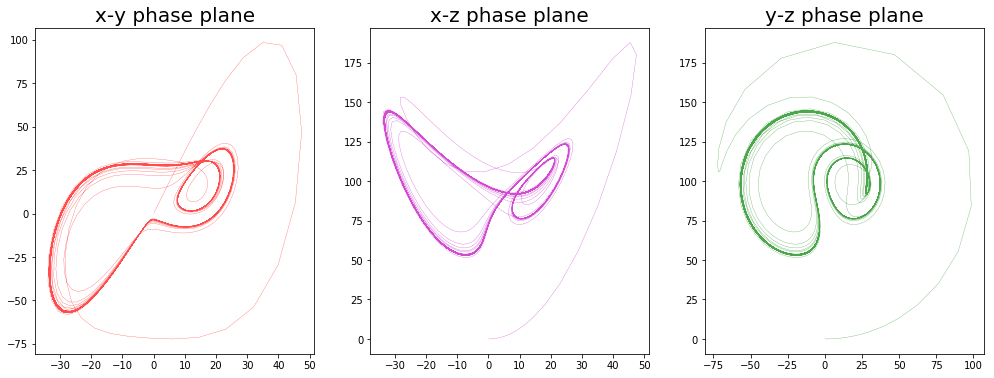
\includegraphics[width=0.8\textwidth]{GraficasTriples3.png}
    \centering
    \label{Grad}
\end{figure}

Al igual que anteriormente, se pedía hacer una animación del comportamiento, sin embargo, esta no fue posible de hacer, ya que el sistema no podía leer los datos apropiadamente, lo que ocasionaba que el ordenador se congelará al poco tiempo de intentar leer los datos.

\end{document}
